\documentclass[
11pt, % The default document font size, options: 10pt, 11pt, 12pt
%codirector, % Uncomment to add a codirector to the title page
]{charter} 




% El títulos de la memoria, se usa en la carátula y se puede usar el cualquier lugar del documento con el comando \ttitle
\titulo{Modelo de migración tecnológica para radares} 

% Nombre del posgrado, se usa en la carátula y se puede usar el cualquier lugar del documento con el comando \degreename
%\posgrado{Carrera de Especialización en Sistemas Embebidos} 
%\posgrado{Carrera de Especialización en Internet de las Cosas} 
%\posgrado{Carrera de Especialización en Intelegencia Artificial}
\posgrado{Maestría en Sistemas Embebidos} 
%\posgrado{Maestría en Internet de las cosas}

% Tu nombre, se puede usar el cualquier lugar del documento con el comando \authorname
\autor{Gonzalo Nahuel Vaca} 

% El nombre del director y co-director, se puede usar el cualquier lugar del documento con el comando \supname y \cosupname y \pertesupname y \pertecosupname
\director{Iván Andrés León Vásquez}
\pertenenciaDirector{INVAP S.E.} 
% FIXME:NO IMPLEMENTADO EL CODIRECTOR ni su pertenencia
\codirector{John Doe} % para que aparezca en la portada se debe descomentar la opción codirector en el documentclass
\pertenenciaCoDirector{FIUBA}

% Nombre del cliente, quien va a aprobar los resultados del proyecto, se puede usar con el comando \clientename y \empclientename
\cliente{Andrés Eduardo Monteverde}
\empresaCliente{INVAP S.E.}

% Nombre y pertenencia de los jurados, se pueden usar el cualquier lugar del documento con el comando \jurunoname, \jurdosname y \jurtresname y \perteunoname, \pertedosname y \pertetresname.
\juradoUno{Nombre y Apellido (1)}
\pertenenciaJurUno{pertenencia (1)} 
\juradoDos{Nombre y Apellido (2)}
\pertenenciaJurDos{pertenencia (2)}
\juradoTres{Nombre y Apellido (3)}
\pertenenciaJurTres{pertenencia (3)}
 
\fechaINICIO{29 de junio de 2022}		%Fecha de inicio de la cursada de GdP \fechaInicioName
\fechaFINALPlan{17 de agosto de 202} 	%Fecha de final de cursada de GdP
\fechaFINALTrabajo{15 de mayo de 2023}	%Fecha de defensa pública del trabajo final


\begin{document}

\maketitle
\thispagestyle{empty}
\pagebreak


\thispagestyle{empty}
{\setlength{\parskip}{0pt}
\tableofcontents{}
}
\pagebreak


\section*{Registros de cambios}
\label{sec:registro}


\begin{table}[ht]
\label{tab:registro}
\centering
\begin{tabularx}{\linewidth}{@{}|c|X|c|@{}}
\hline
\rowcolor[HTML]{C0C0C0} 
Revisión & \multicolumn{1}{c|}{\cellcolor[HTML]{C0C0C0}Detalles de los cambios realizados} & Fecha      \\ \hline
0      & Creación del documento                                 &\fechaInicioName \\ \hline
%1      & Se completa hasta el punto 4 inclusive                 & dd/mm/aaaa \\ \hline
%2      & Se completa hasta el punto 7 inclusive
%		  Se puede agregar algo más \newline
%		  En distintas líneas \newline
%		  Así                                                    & dd/mm/aaaa \\ \hline
%3      & Se completa hasta el punto 11 inclusive                & dd/mm/aaaa \\ \hline
%4      & Se completa el plan	                                 & dd/mm/aaaa \\ \hline
\end{tabularx}
\end{table}

\pagebreak



\section*{Acta de constitución del proyecto}
\label{sec:acta}

\begin{flushright}
Buenos Aires, \fechaInicioName
\end{flushright}

\vspace{2cm}

Por medio de la presente se acuerda con el Mg. Ing. \authorname\hspace{1px} que
su Trabajo Final de la \degreename\hspace{1px} se titulará ``\ttitle'',
consistirá esencialmente en la implementación de un prototipo de
  un procesador de datos de radar hecho en Python, y tendrá un presupuesto preliminar estimado de 600 hs de trabajo y \$200, con fecha de inicio \fechaInicioName\hspace{1px} y fecha de presentación pública \fechaFinalName.

Se adjunta a esta acta la planificación inicial.

\vfill

% Esta parte se construye sola con la información que hayan cargado en el preámbulo del documento y no debe modificarla
\begin{table}[ht]
\centering
\begin{tabular}{ccc}
\begin{tabular}[c]{@{}c@{}}Ariel Lutenberg \\ Director posgrado FIUBA\end{tabular} & \hspace{2cm} & \begin{tabular}[c]{@{}c@{}}\clientename \\ \empclientename \end{tabular} \vspace{2.5cm} \\ 
\multicolumn{3}{c}{\begin{tabular}[c]{@{}c@{}} \supname \\ Director del Trabajo Final\end{tabular}} \vspace{2.5cm} \\
%\begin{tabular}[c]{@{}c@{}}\jurunoname \\ Jurado del Trabajo Final\end{tabular}     &  & \begin{tabular}[c]{@{}c@{}}\jurdosname\\ Jurado del Trabajo Final\end{tabular}  \vspace{2.5cm}  \\
%\multicolumn{3}{c}{\begin{tabular}[c]{@{}c@{}} \jurtresname\\ Jurado del Trabajo Final\end{tabular}} \vspace{.5cm}                                                                     
\end{tabular}
\end{table}




\section{1. Descripción técnica-conceptual del proyecto a realizar}
\label{sec:descripcion}

El proyecto a realizar tiene como cliente al Departamento de ingeniería de
software (DISW) de INVAP S.E. en el marco de la Gerencia de gobierno y defensa.

En la cartera de productos de la empresa se pueden encontrar radares
meteorológicos, de vigilancia primarios y secundarios.
Estos equipos generan un gran volumen de datos que deben ser procesados por
algoritmos complejos con la finalidad de obtener información útil.

Los algoritmos son generados por profesionales especializados en la naturaleza
física y matemática del problema y entregan como producto un modelo de
procesamiento de datos en Python.
Luego, el modelo debe correr dentro de un sistema embebido multiprocesador
asimétrico (MPSoC).
Entonces, se procede a traducir el código al lenguaje de programación C para
lograr su compilación en la arquitectura objetivo.

La traducción del modelo genera los siguientes inconvenientes:

\begin{itemize}
  \item Duplicación de tareas.
  \item Dificultad para depurar: se torna difícil determinar si un
    comportamiento erróneo es producto del diseño del modelo o su traducción al
    lenguaje C.
  \item Baja de confiabilidad: la traducción del código es una fuente de
    posibles errores en el sistema.
\end{itemize}

Con la intención de atenuar estos problemas, se deberá realizar un prototipo que
utilice el algoritmo hecho en Python sin traducir. Esto tendría el beneficio
adicional de aliviar la demanda de programadores C/C++ y buscar personal en una
población mayor.

El proyecto se realizará en un \emph{System on chip} (SoC) Zynq-7000 del fabricante
AMD/Xilinx y tendrá los siguientes componentes:

\begin{itemize}
  \item Generador de datos de radar: se deberá sintetizar en la lógica
    programable del integrado.
  \item Modelo procesador: tendrá que estar realizado en Python y podrá ser
    configurado desde el exterior.
  \item Generador de mensajes ASTERIX: deberá crear los mensajes ASTERIX a
    partir de la información generada.
  \item Generador de telemetría: deberá reportar el estado de funcionamiento
    del sistema con mensajes MQTT.
  \item Backend radar corriendo como servicio.
  \item Creación de una distribución de Linux embebido.
\end{itemize}

En la figura \ref{fig:diagBloques} se puede observar un diagrama en bloques
simplificado del sistema propuesto.

\begin{figure}[htpb]
  \centering 
  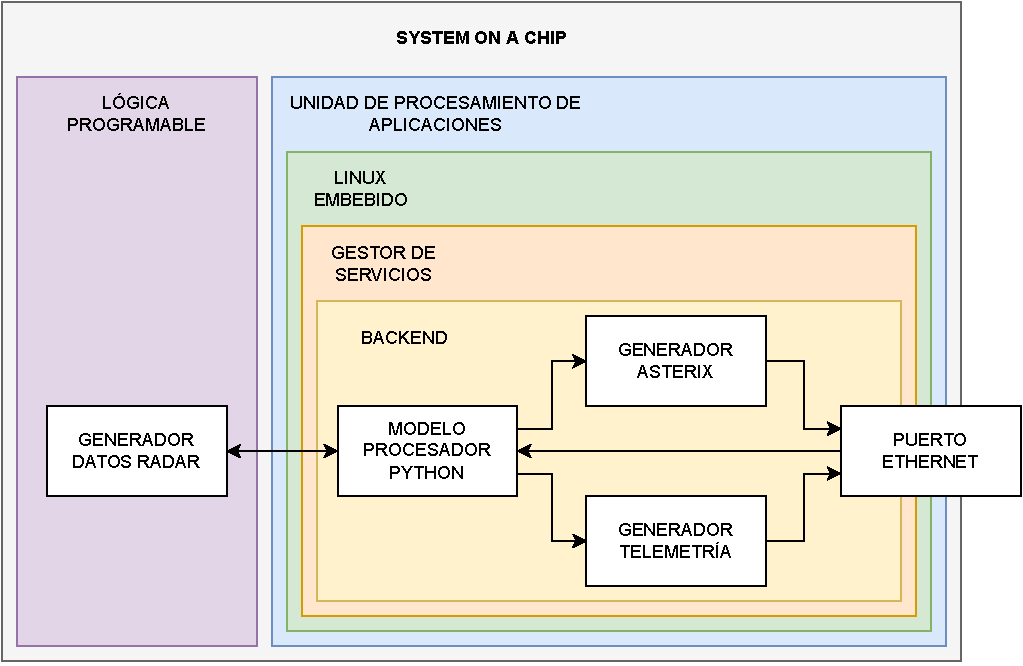
\includegraphics[width=\textwidth]{./Figuras/bloques.pdf}
  \caption{Diagrama en bloques del sistema}
  \label{fig:diagBloques}
\end{figure}


\section{2. Identificación y análisis de los interesados}
\label{sec:interesados}

\begin{table}[ht]
%\caption{Identificación de los interesados}
%\label{tab:interesados}
\begin{tabularx}{\linewidth}{@{}|l|X|X|l|@{}}
\hline
\rowcolor[HTML]{C0C0C0} 
Rol           & Nombre y Apellido & Organización 	  & Puesto \\ \hline
Auspíciate   & Celeste Musso     & \empclientename & Jefa del DISW \\ \hline
Cliente       & \clientename      & \empclientename & Ingeniero de software \\ \hline
Impulsor      & Maximiliano Graf  & \empclientename & Líder de equipo \\ \hline
Responsable   & \authorname       & FIUBA        	  & Alumno \\ \hline
Orientador    & \supname	        & \pertesupname 	& Director del Trabajo final \\ \hline
\end{tabularx}
\end{table}

\section{3. Propósito del proyecto}
\label{sec:proposito}

El propósito de este proyecto es evaluar la posibilidad de realizar un backend
para radares hecho en Python. Con la finalidad de evitar la repetición de
tareas, mejorar la confiabilidad de los sistemas y acceder a una población mayor
de programadores.

\newpage

\section{4. Alcance del proyecto}
\label{sec:alcance}

El presente proyecto incluye:

\begin{itemize}
  \item Crear un esclavo AXI generador de datos de radar.
  \item Crear una distribución de Linux embebido.
  \item Crear un servicio backend radar hecho en Python.
  \item Documentación y manual de usuario.
\end{itemize}

\section{5. Supuestos del proyecto}
\label{sec:supuestos}

Para el desarrollo del presente proyecto se supone que:

\begin{itemize}
	\item Se tendrá acceso a los modelos procesadores de datos de radar.
	\item Se tendrá acceso una captura de datos de radar.
\end{itemize}

\section{6. Requerimientos}
\label{sec:requerimientos}

A continuación se enumeran los requerimientos del proyecto:

\begin{enumerate}
	\item Requerimientos funcionales
		\begin{enumerate}
      \item El sistema se debe implementar en un SoC de Xilinx.
      \item El sistema debe generar un flujo de datos de radar.
      \item El generador de datos debe ser un esclavo AXI en la lógica programable.
			\item La generación de datos debe ser configurable.
			\item El sistema debe procesar los datos y generar mensajes ASTERIX.
      \item El procesador de datos se debe implementar en Python dentro de la
        Unidad de procesamiento de aplicaciones.
      \item El procesador debe correr como servicio dentro del sistema
        operativo.
      \item Se debe crear una distribución de Linux embebido.
			\item Los mensajes ASTERIX se deben transmitir por protocolo ZMQ.
			\item El sistema debe generar datos de telemetría que indiquen su estado
        de funcionamiento.
			\item La telemetría se debe trasmitir por protocolo MQTT.
			\item El sistema debe presentar una interfaz web para ajustar la
        configuración.
      \item Se debe poder visualizar los mensajes ASTERIX y de telemetría.
		\end{enumerate}
	\item Requerimientos de documentación
		\begin{enumerate}
			\item Se debe generar un informe de rendimiento del procesador de datos implementado.
			\item Se debe crear un manual de uso para el esclavo AXI.
      \item Se debe crear un manual de uso para el servicio procesador de datos.
		\end{enumerate}
	\item Se debe proveer una interfaz web para supervisar y configurar el sistema.
\end{enumerate}

\section{7. Historias de usuarios (\textit{Product backlog})}
\label{sec:backlog}

Las historias de usuario reciben una calificación numérica que refleja la
complejidad de su implementación.
A continuación se detallan los valores posibles:

\begin{itemize}
\item 1 punto: la historia demanda un esfuerzo trivial para satisfacerla.
\item 2 puntos: la historia requiere de conocimientos profundos en una
  tecnología particular.
\item 4 puntos: la historia necesita de conocimientos profundos en más de una tecnología.
\item 8 puntos: la historia demanda múltiples tecnologías y debe cumplir con
  requerimientos de rendimiento.
\item 16 puntos: la historia demanda múltiples tecnologías y debe funcionar en
  tiempo real.
\end{itemize}

A continuación se enumeran las historias de usuario:

\begin{itemize}
  \item
    \begin{itemize}
      \item Descripción: como arquitecto de proyectos quiero una interfaz gráfica que me permita
        evaluar el rendimiento del modelo en el sistema embebido.
      \item 8 \emph{History points}: la historia de usuario necesita de
        conocimientos de Python, protocolos ZMQ y HTTP y además se necesita crear
        una página web dentro del sistema embebido. Finalmente, se debe medir el
        rendimiento del sistema.
    \end{itemize}
  \item
    \begin{itemize}
      \item Descripción: como desarrollador de la \emph{Radar Computer} necesito obtener
        telemetría MQTT para actualizar el estado del radar.
      \item 4 \emph{History points}: la historia requiere conocimientos de
        programación concurrente en Python y el manejo del protocolo MQTT.
    \end{itemize}
  \item
    \begin{itemize}
      \item Descripción: como desarrollador de consolas de radar quiero obtener mensajes en
        formato ASTERIX para poder representar las novedades en campo.
      \item 4 \emph{History points}: se necesitan conocimientos de ZMQ, ASTERIX
        y Python.
    \end{itemize}
\end{itemize}

\section{8. Entregables principales del proyecto}
\label{sec:entregables}

Los entregables del proyecto son:

\begin{itemize}
	\item Manual de usuario del generador de datos.
	\item Manual de usuario del servicio de procesamiento de datos.
	\item Código fuente del generador de datos.
	\item Código fuente del servicio de procesamiento de datos.
	\item Informe de rendimiento del servicio de procesamiento de datos.
\end{itemize}


\section{9. Desglose del trabajo en tareas}
\label{sec:wbs}

\begin{consigna}{red}
El WBS debe tener relación directa o indirecta con los requerimientos.  Son todas las actividades que se harán en el proyecto para dar cumplimiento a los requerimientos. Se recomienda mostrar el WBS mediante una lista indexada:

\begin{enumerate}
\item Grupo de tareas 1
	\begin{enumerate}
	\item Tarea 1 (tantas hs)
	\item Tarea 2 (tantas hs)
	\item Tarea 3 (tantas hs)
	\end{enumerate}
\item Grupo de tareas 2
	\begin{enumerate}
	\item Tarea 1 (tantas hs)
	\item Tarea 2 (tantas hs)
	\item Tarea 3 (tantas hs)
	\end{enumerate}
\item Grupo de tareas 3
	\begin{enumerate}
	\item Tarea 1 (tantas hs)
	\item Tarea 2 (tantas hs)
	\item Tarea 3 (tantas hs)
	\item Tarea 4 (tantas hs)
	\item Tarea 5 (tantas hs)
	\end{enumerate}
\end{enumerate}

Cantidad total de horas: (tantas hs)

Se recomienda que no haya ninguna tarea que lleve más de 40 hs. 

\end{consigna}

\section{10. Diagrama de Activity On Node}
\label{sec:AoN}

\begin{consigna}{red}
Armar el AoN a partir del WBS definido en la etapa anterior. 

%La figura \ref{fig:AoN} fue elaborada con el paquete latex tikz y pueden consultar la siguiente referencia \textit{online}:

%\url{https://www.overleaf.com/learn/latex/LaTeX_Graphics_using_TikZ:_A_Tutorial_for_Beginners_(Part_3)\%E2\%80\%94Creating_Flowcharts}

\end{consigna}

\begin{figure}[htpb]
\centering 
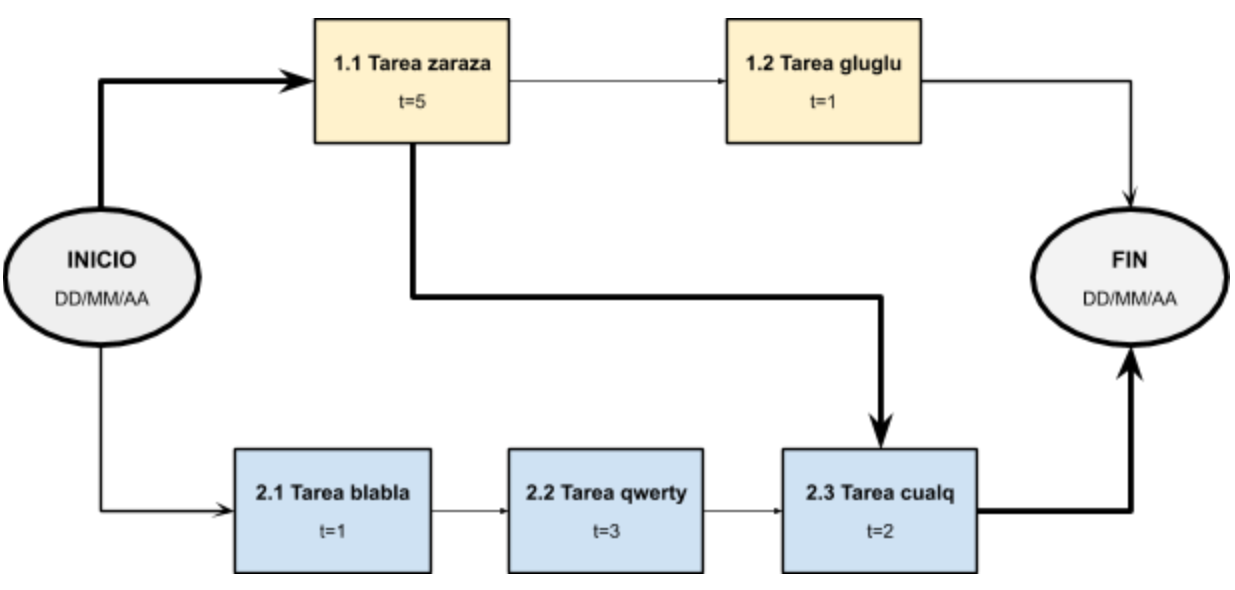
\includegraphics[width=.8\textwidth]{./Figuras/AoN.png}
\caption{Diagrama en \textit{Activity on Node}}
\label{fig:AoN}
\end{figure}

Indicar claramente en qué unidades están expresados los tiempos.
De ser necesario indicar los caminos semicríticos y analizar sus tiempos mediante un cuadro.
Es recomendable usar colores y un cuadro indicativo describiendo qué representa cada color, como se muestra en el siguiente ejemplo:



\section{11. Diagrama de Gantt}
\label{sec:gantt}

\begin{consigna}{red}

Existen muchos programas y recursos \textit{online} para hacer diagramas de gantt, entre los cuales destacamos:

\begin{itemize}
\item Planner
\item GanttProject
\item Trello + \textit{plugins}. En el siguiente link hay un tutorial oficial: \\ \url{https://blog.trello.com/es/diagrama-de-gantt-de-un-proyecto}
\item Creately, herramienta online colaborativa. \\\url{https://creately.com/diagram/example/ieb3p3ml/LaTeX}
\item Se puede hacer en latex con el paquete \textit{pgfgantt}\\ \url{http://ctan.dcc.uchile.cl/graphics/pgf/contrib/pgfgantt/pgfgantt.pdf}
\end{itemize}

Pegar acá una captura de pantalla del diagrama de Gantt, cuidando que la letra sea suficientemente grande como para ser legible. 
Si el diagrama queda demasiado ancho, se puede pegar primero la ``tabla'' del Gantt y luego pegar la parte del diagrama de barras del diagrama de Gantt.

Configurar el software para que en la parte de la tabla muestre los códigos del EDT (WBS).\\
Configurar el software para que al lado de cada barra muestre el nombre de cada tarea.\\
Revisar que la fecha de finalización coincida con lo indicado en el Acta Constitutiva.

En la figura \ref{fig:gantt}, se muestra un ejemplo de diagrama de gantt realizado con el paquete de \textit{pgfgantt}. En la plantilla pueden ver el código que lo genera y usarlo de base para construir el propio.

\begin{figure}[htbp]
\begin{center}
\begin{ganttchart}{1}{12}
  \gantttitle{2020}{12} \\
  \gantttitlelist{1,...,12}{1} \\
  \ganttgroup{Group 1}{1}{7} \\
  \ganttbar{Task 1}{1}{2} \\
  \ganttlinkedbar{Task 2}{3}{7} \ganttnewline
  \ganttmilestone{Milestone o hito}{7} \ganttnewline
  \ganttbar{Final Task}{8}{12}
  \ganttlink{elem2}{elem3}
  \ganttlink{elem3}{elem4}
\end{ganttchart}
\end{center}
\caption{Diagrama de gantt de ejemplo}
\label{fig:gantt}
\end{figure}


\begin{landscape}
\begin{figure}[htpb]
\centering 
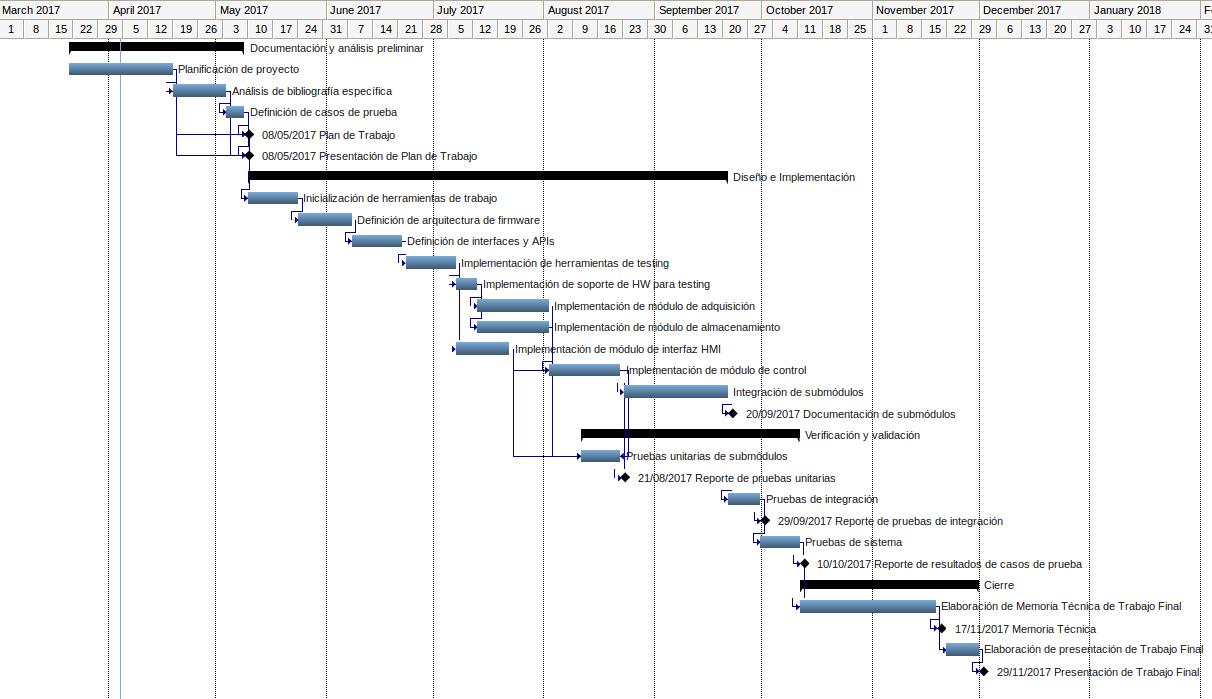
\includegraphics[height=.85\textheight]{./Figuras/Gantt-2.png}
\caption{Ejemplo de diagrama de Gantt rotado}
\label{fig:diagGantt}
\end{figure}

\end{landscape}

\end{consigna}


\section{12. Presupuesto detallado del proyecto}
\label{sec:presupuesto}

\begin{consigna}{red}
Si el proyecto es complejo entonces separarlo en partes:
\begin{itemize}
	\item Un total global, indicando el subtotal acumulado por cada una de las áreas.
	\item El desglose detallado del subtotal de cada una de las áreas.
\end{itemize}

IMPORTANTE: No olvidarse de considerar los COSTOS INDIRECTOS.

\end{consigna}

\begin{table}[htpb]
\centering
\begin{tabularx}{\linewidth}{@{}|X|c|r|r|@{}}
\hline
\rowcolor[HTML]{C0C0C0} 
\multicolumn{4}{|c|}{\cellcolor[HTML]{C0C0C0}COSTOS DIRECTOS} \\ \hline
\rowcolor[HTML]{C0C0C0} 
Descripción &
  \multicolumn{1}{c|}{\cellcolor[HTML]{C0C0C0}Cantidad} &
  \multicolumn{1}{c|}{\cellcolor[HTML]{C0C0C0}Valor unitario} &
  \multicolumn{1}{c|}{\cellcolor[HTML]{C0C0C0}Valor total} \\ \hline
 &
  \multicolumn{1}{c|}{} &
  \multicolumn{1}{c|}{} &
  \multicolumn{1}{c|}{} \\ \hline
 &
  \multicolumn{1}{c|}{} &
  \multicolumn{1}{c|}{} &
  \multicolumn{1}{c|}{} \\ \hline
\multicolumn{1}{|l|}{} &
   &
   &
   \\ \hline
\multicolumn{1}{|l|}{} &
   &
   &
   \\ \hline
\multicolumn{3}{|c|}{SUBTOTAL} &
  \multicolumn{1}{c|}{} \\ \hline
\rowcolor[HTML]{C0C0C0} 
\multicolumn{4}{|c|}{\cellcolor[HTML]{C0C0C0}COSTOS INDIRECTOS} \\ \hline
\rowcolor[HTML]{C0C0C0} 
Descripción &
  \multicolumn{1}{c|}{\cellcolor[HTML]{C0C0C0}Cantidad} &
  \multicolumn{1}{c|}{\cellcolor[HTML]{C0C0C0}Valor unitario} &
  \multicolumn{1}{c|}{\cellcolor[HTML]{C0C0C0}Valor total} \\ \hline
\multicolumn{1}{|l|}{} &
   &
   &
   \\ \hline
\multicolumn{1}{|l|}{} &
   &
   &
   \\ \hline
\multicolumn{1}{|l|}{} &
   &
   &
   \\ \hline
\multicolumn{3}{|c|}{SUBTOTAL} &
  \multicolumn{1}{c|}{} \\ \hline
\rowcolor[HTML]{C0C0C0}
\multicolumn{3}{|c|}{TOTAL} &
   \\ \hline
\end{tabularx}%
\end{table}


\section{13. Gestión de riesgos}
\label{sec:riesgos}

\begin{consigna}{red}
a) Identificación de los riesgos (al menos cinco) y estimación de sus consecuencias:
 
Riesgo 1: detallar el riesgo (riesgo es algo que si ocurre altera los planes previstos de forma negativa)
\begin{itemize}
	\item Severidad (S): mientras más severo, más alto es el número (usar números del 1 al 10).\\
	Justificar el motivo por el cual se asigna determinado número de severidad (S).
	\item Probabilidad de ocurrencia (O): mientras más probable, más alto es el número (usar del 1 al 10).\\
	Justificar el motivo por el cual se asigna determinado número de (O). 
\end{itemize}   

Riesgo 2:
\begin{itemize}
	\item Severidad (S): 
	\item Ocurrencia (O):
\end{itemize}

Riesgo 3:
\begin{itemize}
	\item Severidad (S): 
	\item Ocurrencia (O):
\end{itemize}


b) Tabla de gestión de riesgos:      (El RPN se calcula como RPN=SxO)

\begin{table}[htpb]
\centering
\begin{tabularx}{\linewidth}{@{}|X|c|c|c|c|c|c|@{}}
\hline
\rowcolor[HTML]{C0C0C0} 
Riesgo & S & O & RPN & S* & O* & RPN* \\ \hline
       &   &   &     &    &    &      \\ \hline
       &   &   &     &    &    &      \\ \hline
       &   &   &     &    &    &      \\ \hline
       &   &   &     &    &    &      \\ \hline
       &   &   &     &    &    &      \\ \hline
\end{tabularx}%
\end{table}

Criterio adoptado: 
Se tomarán medidas de mitigación en los riesgos cuyos números de RPN sean mayores a...

Nota: los valores marcados con (*) en la tabla corresponden luego de haber aplicado la mitigación.

c) Plan de mitigación de los riesgos que originalmente excedían el RPN máximo establecido:
 
Riesgo 1: plan de mitigación (si por el RPN fuera necesario elaborar un plan de mitigación).
  Nueva asignación de S y O, con su respectiva justificación:
  - Severidad (S): mientras más severo, más alto es el número (usar números del 1 al 10).
          Justificar el motivo por el cual se asigna determinado número de severidad (S).
  - Probabilidad de ocurrencia (O): mientras más probable, más alto es el número (usar del 1 al 10).
          Justificar el motivo por el cual se asigna determinado número de (O).

Riesgo 2: plan de mitigación (si por el RPN fuera necesario elaborar un plan de mitigación).
 
Riesgo 3: plan de mitigación (si por el RPN fuera necesario elaborar un plan de mitigación).

\end{consigna}


\section{14. Gestión de la calidad}
\label{sec:calidad}

\begin{consigna}{red}
Para cada uno de los requerimientos del proyecto indique:
\begin{itemize} 
\item Req \#1: copiar acá el requerimiento.

\begin{itemize}
	\item Verificación para confirmar si se cumplió con lo requerido antes de mostrar el sistema al cliente. Detallar 
	\item Validación con el cliente para confirmar que está de acuerdo en que se cumplió con lo requerido. Detallar  
\end{itemize}

\end{itemize}

Tener en cuenta que en este contexto se pueden mencionar simulaciones, cálculos, revisión de hojas de datos, consulta con expertos, mediciones, etc.  Las acciones de verificación suelen considerar al entregable como ``caja blanca'', es decir se conoce en profundidad su funcionamiento interno.  En cambio, las acciones de validación suelen considerar al entregable como ``caja negra'', es decir, que no se conocen los detalles de su funcionamiento interno.

\end{consigna}

\section{15. Procesos de cierre}    
\label{sec:cierre}

\begin{consigna}{red}
Establecer las pautas de trabajo para realizar una reunión final de evaluación del proyecto, tal que contemple las siguientes actividades:

\begin{itemize}
	\item Pautas de trabajo que se seguirán para analizar si se respetó el Plan de Proyecto original:
	 - Indicar quién se ocupará de hacer esto y cuál será el procedimiento a aplicar. 
	\item Identificación de las técnicas y procedimientos útiles e inútiles que se emplearon, y los problemas que surgieron y cómo se solucionaron:
	 - Indicar quién se ocupará de hacer esto y cuál será el procedimiento para dejar registro.
	\item Indicar quién organizará el acto de agradecimiento a todos los interesados, y en especial al equipo de trabajo y colaboradores:
	  - Indicar esto y quién financiará los gastos correspondientes.
\end{itemize}

\end{consigna}


\end{document}
